\documentclass[a4paper,10pt]{article}
\usepackage[margin=1in]{geometry}
\usepackage{polski}
\usepackage[utf8x]{inputenc}
\usepackage[unicode]{hyperref}
\usepackage{amssymb}
\usepackage{xifthen}
\usepackage[fleqn]{amsmath}
\usepackage{todonotes}
\usepackage{graphicx}
\usepackage{float}
\usepackage{fullpage}
\usepackage{epstopdf}
\usepackage{multirow}
\usepackage{subfig}
\usepackage[europeanresistors,americaninductors]{circuitikz}
\usetikzlibrary{patterns}
\newcommand{\withtodo}{0}

\def\arraystretch{1.2}

\begin{document}

\begin{table}
  \centering
  \def\arraystretch{1.5}
    \begin{tabular}{|l|l|l|l|} \hline
    Wydział:           & \multicolumn{2}{l|}{Dzień:Poniedziałek 14-17}    &Zespół:  \\
    Fizyki             &    \multicolumn{2}{l|}{Data: 20.03.2017}         &8             \\\hline
    Imiona i nazwiska: &Ocena z przygotowania:  &Ocena ze sprawozdania:   &Ocena końcowa: \\
    Marta Pogorzelska  &                        &                         &                \\
    Paulina Marikin    &                        &                         &\\\hline
    \multicolumn{2}{|l|}{Prowadzący:                 } &\multicolumn{2}{l|}{Podpis:             }  \\\hline
  \end{tabular}
\end{table}

\title{Ćwiczenie 20:\\Badanie właściwości magnetycznych ciał stałych}
\date{}
\maketitle{}

\section{Cel badań}
\paragraph{Zapoznanie się z właściwościami magnetycznymi ciał stałych oraz wyznaczenie temperatury Curie dla rdzenia ferromagnetycznego w transformatorze.}...

\section{Wstęp teoretyczny}
\paragraph{Magnetyzm jest to zjawisko i właściwości fizyczne materii związane z oddziaływaniem ciał poprzez pole magnetyczne. Jego źródłem mogą być naładowane ciała, np.: magnes, pojedyncze cząsteczki lub przewodniki z prądem. Ze względu na sposób oddziaływania danego ciała na zewnętrzne pole magnetyczne można podzielić je na: ferromagnetyki, paramagnetyki, diamagnetyki, anty-ferromagnetyki oraz ferrimagnetyki. Jednostką opisującą stopień w jakim dane ciało wykazuje zdolności magnetyczne jest magnetyzacja lub namagnesowanie - $\vec{M}$. Wyraża się ona wzorem:}

\begin{equation}
\vec{M} =\frac{1}{V} \sum_{i=1}^n \vec{\mu_i}
\end{equation}
\paragraph{gdzie V – objętość, $\vec{\mu_i}$ - elementarny moment magnetyczny.}

\paragraph{Zarówno ferromagnetyki i paramagnetyki posiadają niezerowy moment magnetyczny, ale  tylko ferromagnetyki charakteryzują się istnieniem wewnętrznego pola magnetycznego porządkującego spiny, co objawia się niezerowym namagnesowaniem jego próbek. Podczas gdy spiny paramagnetyków na skutek wyższych temperatur pozostają nieuporządkowane a ich kierunki są całkowicie przypadkowe. W celu uporządkowania układu momentów magnetycznych paramagnetyka można przyłożyć wystarczająco silne zewnętrzne pole magnetyczne albo obniżyć temperaturę danej próbki. Skutkuje to przejściem ciała do fazy ferromagnetycznej. Temperaturą krytyczną przejścia z jednej fazy do drugiej jest tzw. temperatura Curie. W odpowiednio wysokiej temperaturze zarówno uporządkowanie układu jak i namagnesowanie ferromagnetycznej próbki ulegają zanikaniu i następuje przejście do fazy paramagnetycznej zwanym przejściem fazowym drugiego rodzaju.}

\paragraph{Jak wspomniano wyżej, jednym ze sposobów na uporządkowanie układu spinów w paramagnetyku jest przyłożenie zewnętrznego pola magnetycznego. Wielkością charakteryzującą jego reakcję na takie pole jest podatność magnetyczna i wyraża się ona wzorem:}

\begin{equation}
\chi = \frac{M}{H}
\end{equation}

\paragraph{,gdzie H - natężenie pola magnetycznego}

\paragraph{zaś z prawa Curie-Weissa wiemy że:}

\begin{equation}
\chi = \frac{C}{T - \theta}
\end{equation}

\paragraph{gdzie C - stała Curie-Weissa, T - temperatura próbki, $\theta$ - temperatura Curie-Weissa.}

\paragraph{Opisana powyżej podatność jest proporcjonalna do napięcia wtórnego na transformatorze, które będzie mierzone w tym doświadczeniu i indukcyjności opisanej przez zależność:}

\begin{equation}
B = \mu_0 H + \mu_0 M(T)
\end{equation}

W celu wyznaczenia $T_c$ przekształcamy wzór (3) i otrzymujemy:

\begin{equation}
\frac{1}{\chi} = \frac{1}{C} T - \frac{\theta}{C}
\end{equation}

\paragraph{Przedstawiona zależność odwrotności podatności od temperatury jest zależnością liniową.}

\section{Opis układu i metody pomiarowej}
\paragraph{Doświadczenie polegało na wyznaczeniu, za pomocą serii pomiarów napięcia na uzwojeniu wtórnym transformatora w zależności od temperatury,
temperatury Curie dla ferromagnetycznego rdzenia tego transformatora. Po włączeniu komputera i specjalnego programu należało rozgrzać grzałkę najpier
w do 20\% jej mocy i odnotować kilka pomiarów napięcia dla danej temperatury. Następnie ustawiono moc grzałki na 70\%, odnotowano kilka pomiarów dla n
owej temperatury, a następnie pozostawiono układ na ok 1,5 godziny w celu osiągnięcia przez grzałkę oczekiwanej temperatury. Po upływie czasu dokonywa
no pomiarów co minutę, za każdym razem podwyższając moc grzałki o 1\% i powtarzając czynność aż moc wyniesie 100\%. Na koniec obniżono moc grzałki w c
elu wychłodzenia układu i po odczekaniu chwili wyłączono komputer oraz odłączono układ od prądu.\\}

\begin{figure}[H]
\center
\includegraphics[width=0.5\textwidth]{uklad.png}
\end{figure}

\paragraph{Na przedstawiony powyżej układ użyty w doświadczeniu składa się: źródło prądu zmiennego, uzwojenie pierwotne transformatora $n_p$, uzwojenie wtórne transformatora $n_w$, ferromagnetyczny rdzeń, termometr elektroniczny podłączony do próbki, woltomierz cyfrowy oraz grzałka. Całość układu podłączona jest do komputera ze specjalnym oprogramowaniem, dzięki któremu można zmieniać moc grzałki oraz który archiwizuje otrzymane wyniki i nanosi je na wykres zależności napięcia od temperatury.}...

\section{Wyniki pomiarów}

\begin{tabular}{lrrrr}
\hline
{} &T($^\circ$C)&delta T($^\circ$C)&U[mV]&delta U[mV]\\
\hline
0  &   20.0 &  5.100 &  452.0 &  11.780 \\
1  &   95.0 &  5.475 &  452.0 &  11.780 \\
2  &  117.0 &  5.585 &  449.0 &  11.735 \\
3  &  122.0 &  5.610 &  447.0 &  11.705 \\
4  &  128.0 &  5.640 &  442.0 &  11.630 \\
5  &  133.0 &  5.665 &  436.0 &  11.540 \\
6  &  137.0 &  5.685 &  435.0 &  11.525 \\
7  &  141.0 &  5.705 &  429.0 &  11.435 \\
8  &  144.0 &  5.720 &  422.0 &  11.330 \\
9  &  147.0 &  5.735 &  416.0 &  11.240 \\
10 &  150.0 &  5.750 &  407.0 &  11.105 \\
11 &  153.0 &  5.765 &  396.0 &  10.940 \\
12 &  156.0 &  5.780 &  383.0 &  10.745 \\
13 &  159.0 &  5.795 &  361.0 &  10.415 \\
14 &  162.0 &  5.810 &  334.0 &  10.010 \\
15 &  165.0 &  5.825 &  301.0 &   9.515 \\
16 &  168.0 &  5.840 &  262.0 &   8.930 \\
17 &  170.0 &  5.850 &  221.0 &   8.315 \\
18 &  173.0 &  5.865 &  183.0 &   7.745 \\
19 &  176.0 &  5.880 &  146.0 &   7.190 \\
20 &  179.0 &  5.895 &  111.0 &   6.665 \\
21 &  183.0 &  5.915 &   78.0 &   6.170 \\
22 &  186.0 &  5.930 &   57.0 &   5.855 \\
23 &  189.0 &  5.945 &   42.0 &   5.630 \\
24 &  192.0 &  5.960 &   34.0 &   5.510 \\
25 &  195.0 &  5.975 &   29.0 &   5.435 \\
26 &  198.0 &  5.990 &   25.0 &   5.375 \\
27 &  201.0 &  6.005 &   22.0 &   5.330 \\
28 &  203.0 &  6.015 &   21.0 &   5.315 \\
29 &  206.0 &  6.030 &   20.0 &   5.300 \\
30 &  208.0 &  6.040 &   19.0 &   5.285 \\
31 &  211.0 &  6.055 &   18.0 &   5.270 \\
\hline
\end{tabular}

\section{Analiza pomiarów}

\begin{figure}[H]
  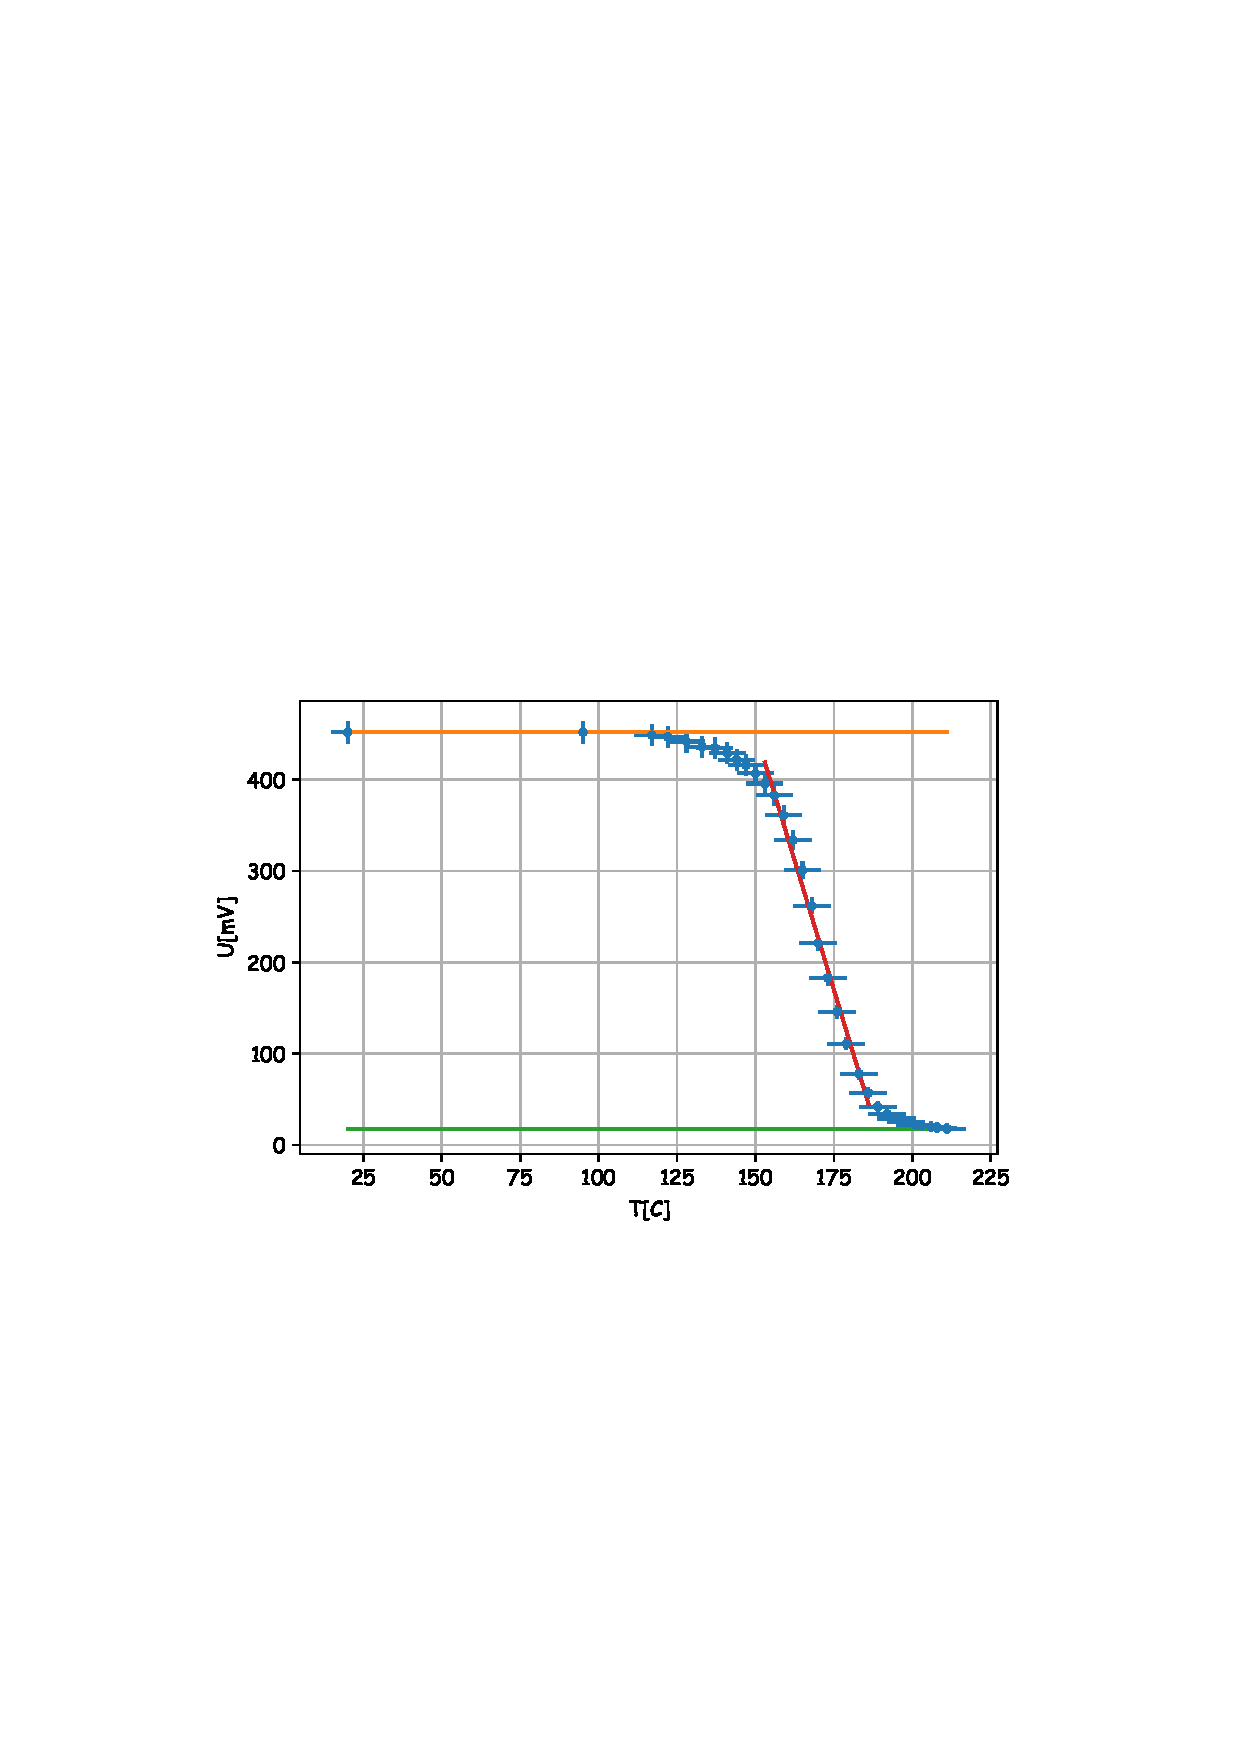
\includegraphics{./Curie_proste.png}
  \caption{Wykres zależności $U(T)$ z prostymi dla maksymalnego i minimalnego napięcia oraz prostą dopasowaną do najostrzejszej części wykresu}
\end{figure}

Na wykresie 1 wartości napięcia utrzymują mniej-więcej(w zakresie błędów pomiarowych) stały poziom dla temperatur poniżej 128$^\circ$C (452mV
- wynikający z maksymalnego namagnesowania rdzenia)i temperatur powyżej 201$^\circ$C (18mV). 
Prosta dopasowana do pomiarów z najwyższym spadkiem leży najpierw
poniżej, a następnie powyżej punktów pomiarowych i przechodzi przez nie w temperaturze $T = 170^\circ C$, którąz w związku z tym możemy uznać za temperature Curie.

\begin{figure}[H]
  \includegraphics{./Curie_odwrotnosc.png}
  \caption{Wykres zależności $\frac{1}{U}$(T) dla fazy paramagnetyka}
\end{figure}
\begin{figure}[H]
  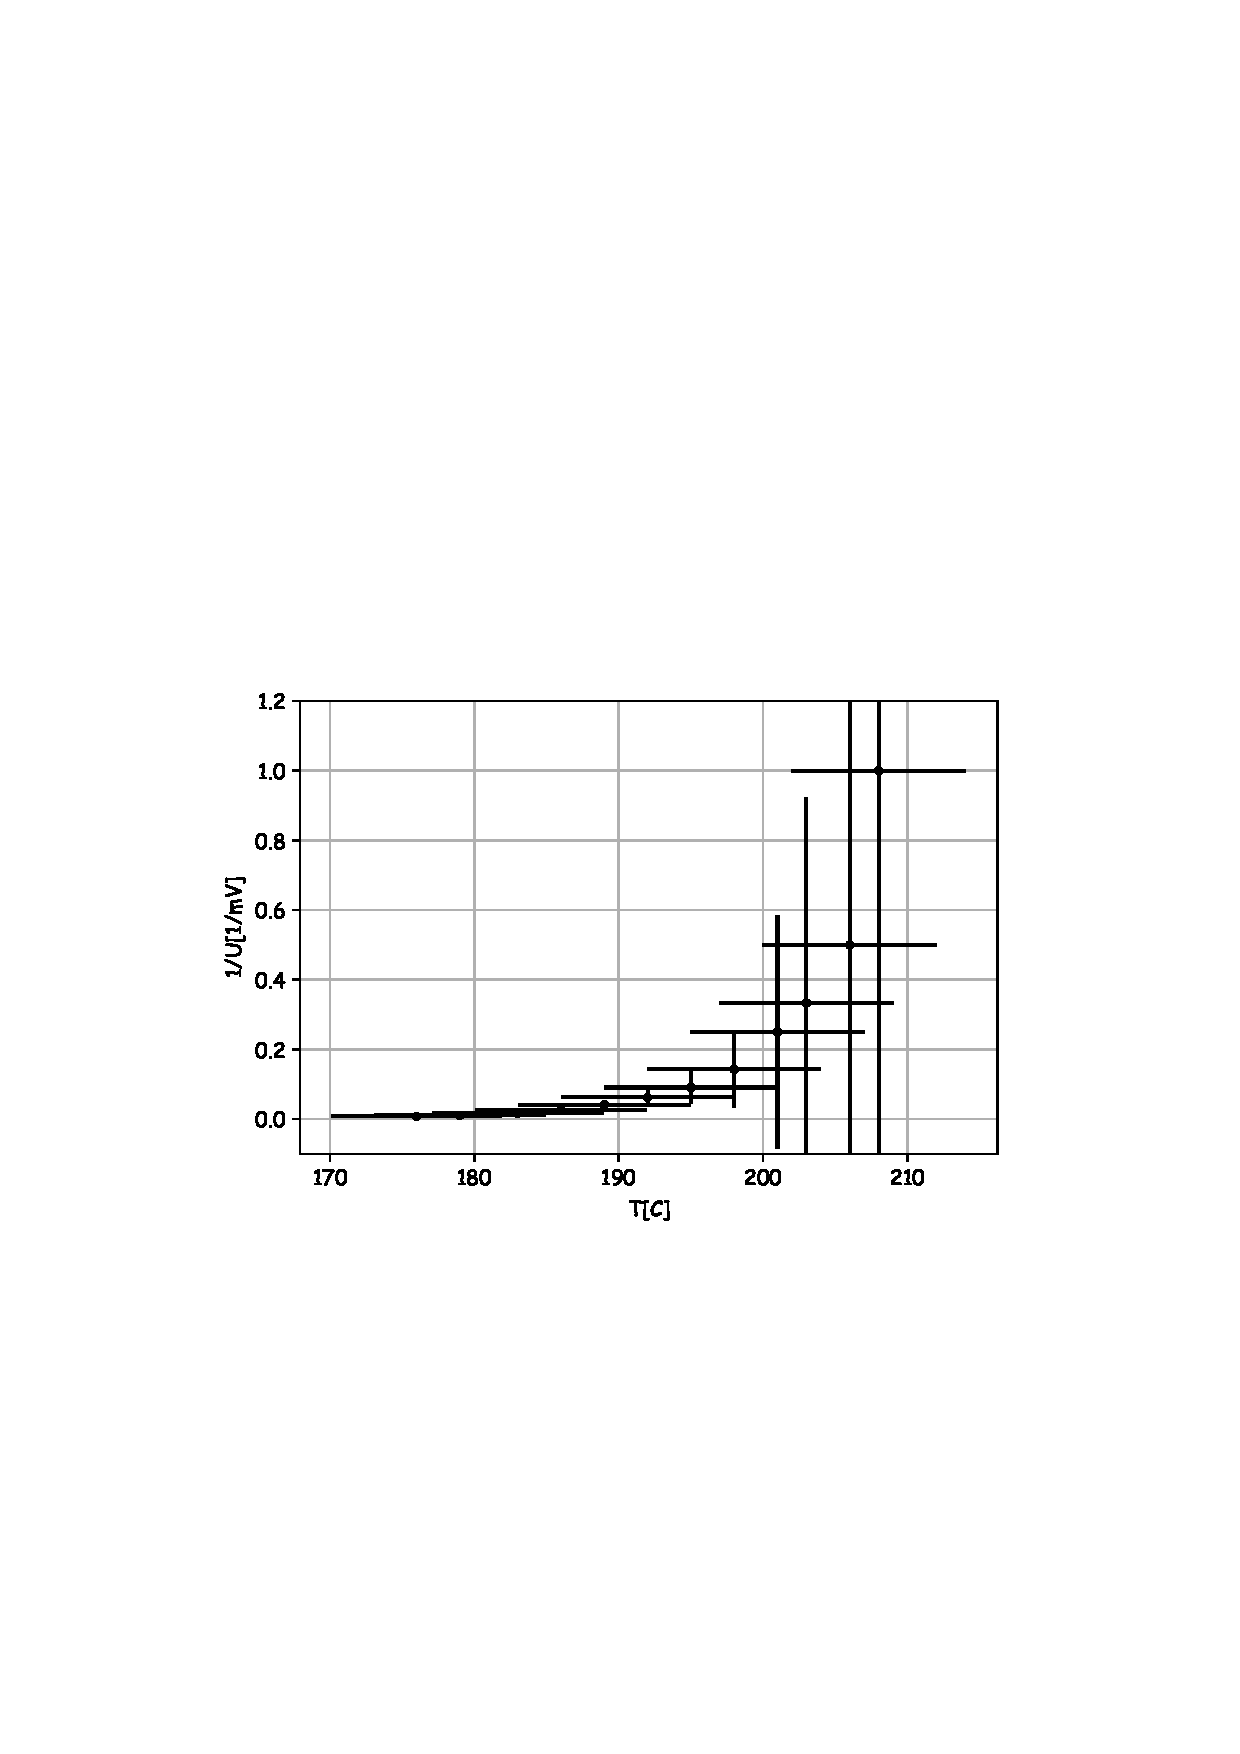
\includegraphics{./Curie_odjete.png}
  \caption{Wykres zależności $\frac{1}{U-U_{min}}$(T) dla fazy paramagnetyka}
\end{figure}

Zgodnie z prawem Curie-Weissa wykres 2 powinien być linią prostą, jednak choć dopasowanie prostej w zakresie niepewności jest możliwe, skala niepewności w porównaniu do wielkości pomiarów jest na tyle duża że przed potwierdzeniem tezy należało by popracować nad dokładnością pomiarów a następnie powtórzyć doświadczenie.
\section{Analiza niepewności}

Niepewności pomiarów temperatury została wyliczona jako iloczyn danego pomiaru i klasy urządzenia pomiarowego(0.005) + 5$^\circ$C
Niepewności napięcia wyliczono tożsamą metodą dla klasy 0.01 i dodając 1mV.
Metody użyte w analizie wyników nie były ściśle analityczne, co nie pozwala na bezpośrednie wyliczenie niepewności jednak można ją oszacować jako przedział maksymalnego spadku na $18c^\circ$
Pozostałe niepewności na wykresach zostały wyliczone przy użyciu metody propagacji niepewności.
 
\section{Wnioski}
Wyznaczona temperatura Curie wynosi $170(18)C^\circ$, jednak biorąc pod uwagę niepewność temperatury Curie, metoda, której użyto w tym doświadczeniu jest niedokładna i  nie nadaje się do jej wyznaczenia.
Zależności wyliczone na podstawie wzoru (4) i przedstawione na wykresie 2 pasują do wykresu jednak niepewności punktów pomiarowych są zbyt duże by stanowiło to potwierdzenie tezy.Wykres 3 nienadaje się do analizy ze względu na zbyt duże niepewności i nie pozwalaja na potwierdzenie bądź odrzucenie tezy. 


\end{document}
